%%
%% Meta: Befragung für Datenanalyse
%% a) Fragen des Bogen von B. Heimgartner
%% b) Angereichert mit Fragen von Marthaler S 398 Aufg 2
%% c) ... weitere ...

\input{bmsLayoutPage}

%%%%%%%%%%%%%%%%%%%%%%%%%%%%%%%%%%%%%%%%%%%%%%%%%%%%%%%%%%%%%%%%%%
\renewcommand{\metaHeaderLine}{Arbeitsblatt}
\renewcommand{\arbeitsblattTitel}{Fragebogen zur Datenanalyse}
    \usepackage{footnote}
    \makesavenoteenv{tabular}



\newcounter{befrageCounter}
\setcounter{befrageCounter}{1}

\newenvironment{befrage}{\begin{tabular}{rp{11.5cm}p{4cm}   }\arabic{befrageCounter}.\stepcounter{befrageCounter}&}{\end{tabular}}


\begin{document}%%


\arbeitsblattHeader{}

\begin{tabular}{|l|l|l|}
\hline
&&\\[-1em]
UE\footnote{UE: Untersuchungseinheit dient der Anonymisierung}:
.......... & Name: .................................................................................. & Klasse: ...................\\
\hline%%
\end{tabular}

\begin{tabular}{lp{0.5cm}p{13cm}}
Hinweise && \textbullet Fragebogen kann anonym ausgefüllt werden.\\
         && \textbullet Angegebene Namen werden nur dem aktuellen Klassenzug angezeigt.\\
         && \textbullet Bei $\bigcirc$ handelt es sich um Einfachantworten,\\
         && \textbullet bei $\square$ sind Mehrfachnennungen möglich (Nr. 6).\\
\end{tabular}


\begin{befrage} 
   Ihr Alter & .......... [Jahre]
\end{befrage}

\begin{befrage} 
   Ihre Körpergröße & .......... [cm]
\end{befrage}


\begin{befrage} 
   Marke Ihres Haupt-Mobiltelefons &
   \begin{tabular}[t]{l}
   $\bigcirc$ Samsung\\
   $\bigcirc$ Apple (iPhone)\\
   $\bigcirc$ Huawei\\
   $\bigcirc$ Xiaomi\\
   $\bigcirc$ Google\\
   $\bigcirc$ LG\\
   $\bigcirc$ HTC\\
   $\bigcirc$ Nokia\\
   $\bigcirc$ Oppo\\
   $\bigcirc$ Oneplus\\
   $\bigcirc$ Blackberry\\
   $\bigcirc$ Microsoft\\
   $\bigcirc$ Sony\\
   $\bigcirc$ anderes: ..........
   \end{tabular}
\end{befrage}


\begin{befrage}
 Anzahl Mitarbeiter/innen Ihres Betriebs in der Schweiz.   & .......... Mitarbeiter/innen
\end{befrage}


\begin{befrage}
  Wie viel Zeit in Minuten wenden Sie durchschnittlich für Ihre Hausaufgaben in allen Fächern pro Woche auf?  & .......... Minuten
\end{befrage}


\begin{befrage}
 Aus welchen Gründen besuchen Sie die BMS? (Mehrfachnennungen sind möglich!)   &
  \begin{tabular}[t]{p{4cm}}
   $\square$ Späteres Studium\\
   $\square$ Berufsaussichten\\
   $\square$ Verdienstmöglichkeiten\\
   $\square$ Auf Wunsch der Eltern\\
   $\square$ Alle Möglichkeiten offen halten\\
   $\square$ andere: ..........
   \end{tabular}
\end{befrage}


\begin{befrage}
  Beurteilen Sie Ihre derzeitige Motivation für die BM  &
   \begin{tabular}[t]{l}
   $\bigcirc$ Sehr groß\\
   $\bigcirc$ groß\\
   $\bigcirc$ gering\\
   $\bigcirc$ keine
   \end{tabular}
\end{befrage}


\begin{befrage}
  Um wie viel Uhr sind Sie gestern (bzw. heute) schlafen gegangen?(24 h Format)  &
  Um .......... Uhr.
\end{befrage}


\begin{befrage}
  Welche Mathematiknote hatten Sie bei der Aufnahmeprüfung & Note: ..........
\end{befrage}

\begin{befrage}
 Welches ist Ihre Lieblingsfarbe  & ..........
\end{befrage}

\begin{befrage}
 Wie hoch ist Ihr Puls im Moment?
(Messen Sie ihn!)  & .......... %% Absichtlich keine Maßangabe
\end{befrage}

\begin{befrage}
 Wie hoch war die höchste Temperatur in Ihren Sommerferien?  & .......... ${}^0C$
\end{befrage}

\begin{befrage}
 Wie teuer war Ihr letzter Besuch beim Coiffeur?  & .......... CHF
\end{befrage}

\begin{center}
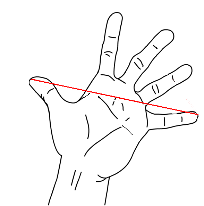
\includegraphics[width=4cm]{img/hand.png}
\end{center}

\begin{befrage}
Wie groß ist die Handspanne Ihrer linken Hand?
Ausgehend von der gespreizten Hand, die Distanz zwischen Fingerspitze des kleinen Fingers und der Spitze des Daumens.  &  .......... cm
\end{befrage}

\subsection*{Fragen aus dem Lehrmittel}
Marthaler S. 398 Kap. 26 Übungen Aufgabe 2:

\begin{befrage}
 Umfang Ihres linken Handgelenks (UHlinks)  & .......... cm
\end{befrage}

\begin{befrage}
 Umfang Ihres rechten Handgelenks (UHrechts)  & .......... cm
\end{befrage}

\begin{befrage}
 Händigkeit  &
 \begin{tabular}[t]{l}
   $\bigcirc$ L\\
   $\bigcirc$ R\\
   $\bigcirc$ L/R gleichermaßen\\
   \end{tabular}
\end{befrage}

\begin{befrage}
  Mund: Wie viele Milliliter Wasser haben in Ihrem geschlossenen Mund Platz? & .......... ml
\end{befrage}

\begin{befrage}
  Gewicht Ihres Portemonnaies & ......... gr
\end{befrage}

\begin{befrage}
 Einkommen (monatlich / brutto) & .......... CHF
\end{befrage}

\begin{befrage}
 Wetterempfindlichkeit &
 \begin{tabular}[t]{l}
   $\bigcirc$ stark\\
   $\bigcirc$ mittel\\
   $\bigcirc$ schwach\\
   $\bigcirc$ nicht vorhanden\\
   \end{tabular}
\end{befrage}


\end{document}
